\documentclass{article}
\usepackage{xcolor}
\usepackage{float}
\parindent0pt
\usepackage[pagebackref=true,colorlinks,linkcolor=blue,citecolor=green!80!black]{hyperref}
\usepackage{amssymb}
\usepackage{amsmath}
\usepackage{verbatim}
\usepackage{fancyvrb}
\usepackage{xcolor}
\usepackage{ragged2e}
\newcommand*\justifyv{%
\fontdimen2\font=0.4em
\fontdimen3\font=0.2em
\fontdimen4\font=0.1em
\fontdimen7\font=0.1em
\hyphenchar\font=`\-
}
\usepackage{fancyhdr}
%\usepackage{url}
\usepackage[compress]{cite} 
%باید دوبار خروجی بگیرید.
%\usepackage[numbers,sort&compress]{natbib}
\usepackage{graphicx}
\usepackage{xepersian}
\settextfont{Yas}
\newcommand{\PRL}[1]{\RL{\Parsifont #1}}
\DefineVerbatimEnvironment{rtlverbatim}{Verbatim}{commandchars=+\[\]}
\newfontfamily\Parsifont[Script=Arabic]{XB Niloofar}
\newcommand{\prl}[1]{\RL{\Parsifont #1}}
\newcommand{\pdflatex}{P\!\!\reflectbox{\raisebox{-1mm}{{\small D}}}F\LaTeX}
\pagestyle{fancy}
\fancyhf{}
\rhead[OR]{\lr{\thepage}}
\lhead[EL]{\lr{\leftmark}}
\renewcommand{\headrulewidth}{1pt}
\renewcommand{\footrulewidth}{1pt}
\fancyfoot[C]{{\lr{\color{green!50!black} By Shapour Madadpour}}}
\begin{document}
\begin{latin}\tableofcontents
\paragraph{\color{red!50!black} version: 1.3}
\paragraph{\color{red!50!black}10 March 2019}
\section{\lr{alpha-persian.bst with \XeLaTeX}}	\label{12}
\noindent
Bib style ``alpha-persian", Persian (farsi)  version of alpha.bst (RTL and LTR references).\\
\begin{Verbatim}[fontsize=\bf,commandchars=\^\#\*,baselinestretch=1,firstnumber=1,formatcom=\color{red!50!black}]
By: Shapour Madadpour
E-mail: madad_sh@yahoo.com
\end{Verbatim}
{\color{red}$\hookrightarrow$ First Compile:} XeLaTex-BibTeX-XeLaTex-XeLaTex\\
With this compile, persian references set at the end of latin references.\\
{\tt\color{blue} Sample:}
\end{latin}	
\begin{Verbatim}[numbers=left,fontsize=\bf,commandchars=\^\#\*,baselinestretch=1,firstnumber=1,formatcom=\color{green!50!black}]
@article{karamzadeh2012prime,
author={Karamzadeh, Omid Ali Shahny},
title={The Prime Avoidance Lemma Revisited},
key={7},
journal={Kyungpook mathematical journal},
volume={52},
number={2},
pages={149^raisebox#.5mm--* ^!^!^!153},
year={2012},
quotation={1},
publisher={Department of Mathematics, Kyungpook National University}
}
@phdthesis{mmm,
title={^prl#فضای توپولوژی*},
author={^prl# رضایی علی‌آباد,علی*},
journal={Kyungpook mathematical journal},
pages={1163^raisebox#.5mm--* ^!^!^!1171},
LANGUAGE ={Persian},
mlabel={^prl#ا.م.ف*},
murl={http://www.w3.org/TR/prov-o/},
series={second series},
year={2002},
chapter={5},
quotation={1},
school={^prl#دانشگاه چمران اهواز*},
}
\end{Verbatim}
\begin{figure}[H]
\centering
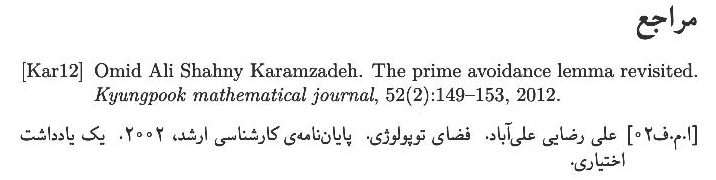
\includegraphics[width=\textwidth,height=3cm]{image/sh11}
\end{figure}
\begin{latin}\noindent
{\color{red}$\hookrightarrow$ Second Compile:} XeLaTex-BibTeX 8 bit-XeLaTex-XeLaTex\\
{\tt txs:///xelatex |bibtex8 -W -c cp1256fa %.aux| txs:///xelatex|txs:///       
xelatex.}\\
With this compile, latin references set at the end of  persian references.\\
{\tt\color{blue} Sample:}
\end{latin}	
\begin{figure}[H]
\centering
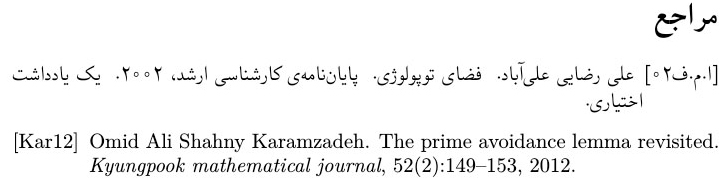
\includegraphics[width=\textwidth,height=3cm]{image/sht}
\end{figure}
\begin{latin}\noindent
{\tt {\color{red}$\hookrightarrow$ quotation mark for title automatically.}}\\
{\tt\color{blue} Sample:}
\end{latin}
\begin{Verbatim}[numbers=left,fontsize=\bf,commandchars=\^\#\*,baselinestretch=1,firstnumber=1,formatcom=\color{green!50!black}]
@article{karamzadeh2012prime,
author={Karamzadeh, Omid Ali Shahny},
title={The Prime Avoidance Lemma Revisited},
key={7},
journal={Kyungpook mathematical journal},
volume={52},
number={2},
pages={149^raisebox#.5mm--* ^!^!^!153},
year={2012},
quotation={1},
madadurltest={1},
murl={http://www.w3.org/TR/prov-o/},
publisher={Department of Mathematics, Kyungpook National University}
}
@phdthesis{mmm,
title={^prl#فضای توپولوژی*},
author={^prl#رضایی علی‌آباد,علی*},
journal={Kyungpook mathematical journal},
pages={1163^raisebox#.5mm--* ^!^!^!1171},
LANGUAGE={Persian},
mlabel={^prl#ا.م.ف*},
madadurltest={1},
quotation={1},
murl={http://www.w3.org/TR/prov-o/},
series={second series},
year={2002},
chapter={5},
school={^prl#دانشگاه چمران اهواز*},
}
\end{Verbatim}
\begin{figure}[H]
\centering
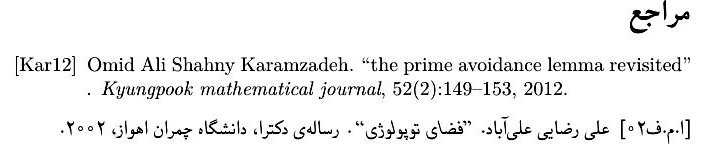
\includegraphics[width=\textwidth,height=3cm]{image/sh2}
\end{figure}
\begin{latin}\noindent
{\tt {\color{red}$\hookrightarrow$ with or without link for title  automatically with hyperref\\ package.}}\\
{\tt\color{blue} Sample:}
\begin{Verbatim}[numbers=left,fontsize=\bf,commandchars=\^\#\*,baselinestretch=1,firstnumber=1,formatcom=\color{green!50!black}]
\usepackage[pagebackref=true,colorlinks,linkcolor=blue]{hyperref}
\usepackage{xepersian}
\settextfont{Yas}
\end{Verbatim}
\end{latin}
\begin{figure}[H]
\centering
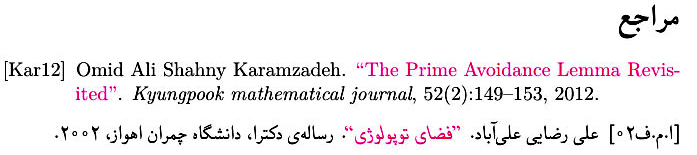
\includegraphics[width=\textwidth,height=3cm]{image/sh3}
\end{figure}
\begin{latin}\noindent
{\tt {\color{red}$\hookrightarrow$ in addition to url with url and  hyperref packages,  it can\\ have url feild without them.}}\\
{\tt\color{blue} Sample with hyperref package:}
\end{latin}
\begin{Verbatim}[numbers=left,fontsize=\bf,commandchars=\^\#\*,baselinestretch=1,firstnumber=1,formatcom=\color{green!50!black}]
@article{karamzadeh2012prime,
author={Karamzadeh, Omid Ali Shahny},
title={The Prime Avoidance Lemma Revisited},
key={7},
journal={Kyungpook mathematical journal},
volume={52},
number={2},
pages={149--153},
year={2012},
quotation={1},
url={http://www.w3.org/TR/prov-o/},
publisher={Department of Mathematics, Kyungpook National University}
}
@phdthesis{mmm,
title={^prl#فضای توپولوژی*},
author={^prl#رضایی علی‌آباد,علی*},
journal={Kyungpook mathematical journal},
pages={1163^raisebox#.5mm--* ^!^!^!1171},
LANGUAGE={Persian},
mlabel={^prl#ا.م.ف*},
madadurltest={1},
quotation={1},
murl={http://www.w3.org/TR/prov-o/},
series={second series},
year={2002},
url={http://www.w3.org/TR/prov-o/},
chapter={5},
school={^prl#دانشگاه چمران اهواز*},
}
\end{Verbatim}
\begin{figure}[H]
\centering

\includegraphics[width=\textwidth,height=3cm]{image/sh4}
\end{figure}

\begin{latin}
{\tt {\color{blue}Sample without url and  hyperref packages:}}
\end{latin}\noindent
\begin{figure}[H]
\centering
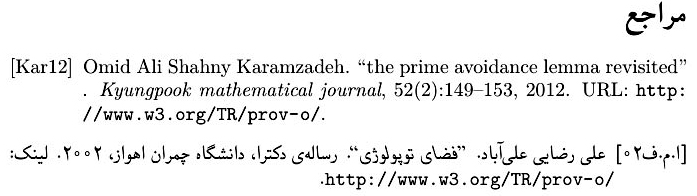
\includegraphics[width=\textwidth,height=3.5cm]{image/sh5}
\end{figure}

\begin{latin}
{\tt{\color{red}$\hookrightarrow$ issn+isbn+doi+et~al in english and persian bibstyle:}}\\
{ isbn Added. It Writes in Persian style \rl{"شابک``}.\\
 issn Added. It Writes in Persian style \rl{"شاپا``}.\\
doi Added. It Writes in Persian style\rl{"شناسه‌ی دیجیتال``}.}\\
{\rl{"شابک``}, \rl{"شاپا``} and \rl{"شناسه‌ی دیجیتال``} for {\color{blue} first time} in persian bib style}\\
{\tt\color{blue} Sample:}
\begin{Verbatim}[numbers=left,fontsize=\bf,commandchars=\&\#\*,baselinestretch=1,firstnumber=1,formatcom=\color{green!50!black}]
@inbook{d,
AUTHOR={&prl#مددپور, شاپور* and &prl#مددپور, محمدحسین* and &prl#سایرین*},
mlabel={&prl#مدد$^+$*},
TITLE={&prl#همریختی و بروریختی در حلقه‌ها*},
JOURNAL={&prl#مجله‌ی گراف فارس*},
VOLUME ={1},
YEAR={1395},
MONTH={&prl#بهار*},
PAGES={39&raisebox#.5mm--* &!&!&!43},
quotation={1},
LANGUAGE={Persian},
url={http://www.w3.org/TR/prov-o/},
doi={01.1000/doi-0121},
isbn={123456789000},
edition={&prl#دوم*},
series={&prl#سری دوم*},
number={10},
chapter={5},
madadurltest={1},
murl={http://www.w3.org/TR/prov-o/},
publisher={&prl#انتشارات دل آهنگ*},
note={&prl#یک یادداشت اختیاری در این‌جا می‌توانید وارد کنید*},
address={&prl#آدرس منتشر کننده*},
}
@book{kuznetsov1998elements,
title={Elements of applied bifurcation theory},
volume={112},
madadurltest={1},
year={1998},
edition={third},
publisher={Springer Verlag},
murl={http://www.w3.org/TR/prov-o/},
isbn={123456789000},
number={10},
pages={10&raisebox#.5mm--* &!&!&!19},
series={second series},
chapter={5},
issn={1111-2222},
doi={01.1000/doi-0121},
editor={Kuznetsov, Y.A. and edward, Y.A.},
address={The address of the publisher},
}
\end{Verbatim}
\end{latin}
\begin{figure}[H]
\centering
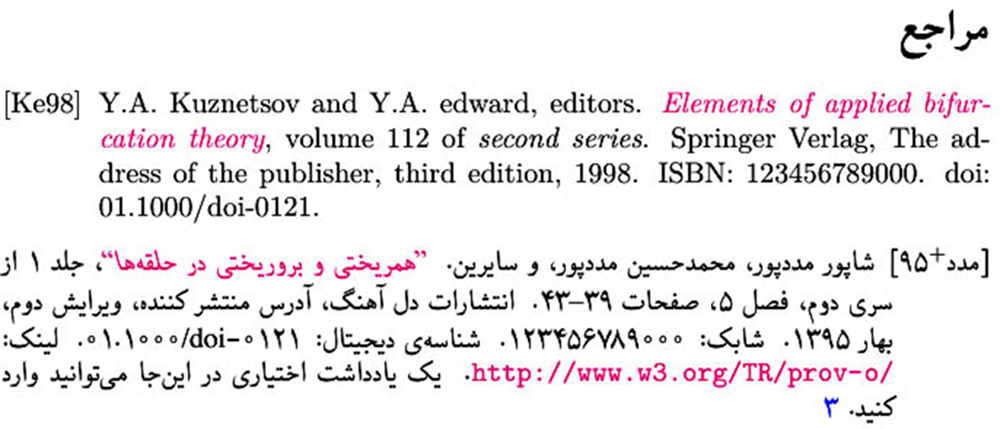
\includegraphics[width=\textwidth,height=5.5cm]{image/sh6}
\end{figure}
\begin{latin}
{\tt {\color{red}$\hookrightarrow$ Flexible for each defined label with appropriative field.}}\\
{\tt\color{blue} Sample:}
\end{latin}
\begin{Verbatim}[numbers=left,fontsize=\bf,commandchars=\&\#\*,baselinestretch=1,firstnumber=1,formatcom=\color{green!50!black}]
slabel={$\checkmark\checkmark\checkmark$},
OR
slabel={$\spadesuit$},
OR
slabel={$\clubsuit$},
\end{Verbatim}
\begin{figure}[H]
\centering
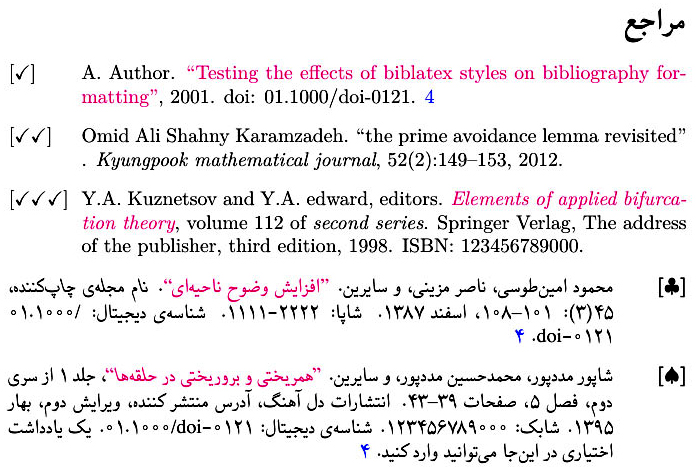
\includegraphics[width=\textwidth,height=8cm]{image/sh7}
\end{figure}

\begin{latin}
{\tt{\color{red}$\hookrightarrow$  in addition to general label, we can choose numbering label.}}\\
{\tt\color{blue} Sample:}
\begin{Verbatim}[numbers=left,fontsize=\bf,commandchars=\&\#\*,baselinestretch=1,firstnumber=1,formatcom=\color{green!50!black}]
slabel={1},
OR
slabel={2},
OR
slabel={3},
OR
slabel={4},
\end{Verbatim}
\end{latin}
\begin{figure}[H]
\centering
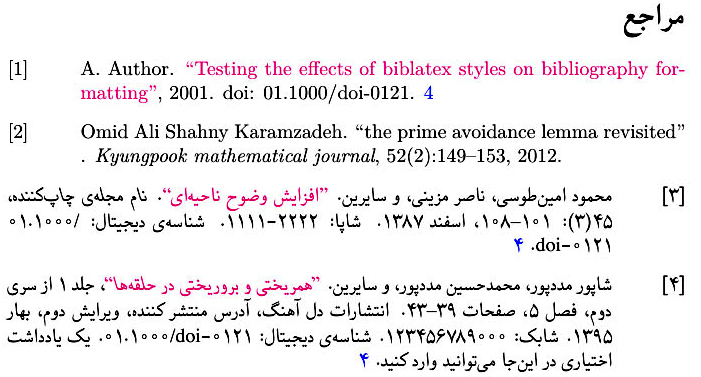
\includegraphics[width=\textwidth,height=7cm]{image/sh8}
\end{figure}
\begin{latin}
{\tt {\color{red}$\hookrightarrow$ Compatible with  hyperref, url, natbib and cite packages.}}
\end{latin}
\begin{latin}
\begin{verbatim}
\usepackage[numbers]{natbib}
\usepackage[compress]{cite} 
\end{verbatim}
{\tt\color{blue} Sample:}
\end{latin}
\begin{figure}[H]
\centering
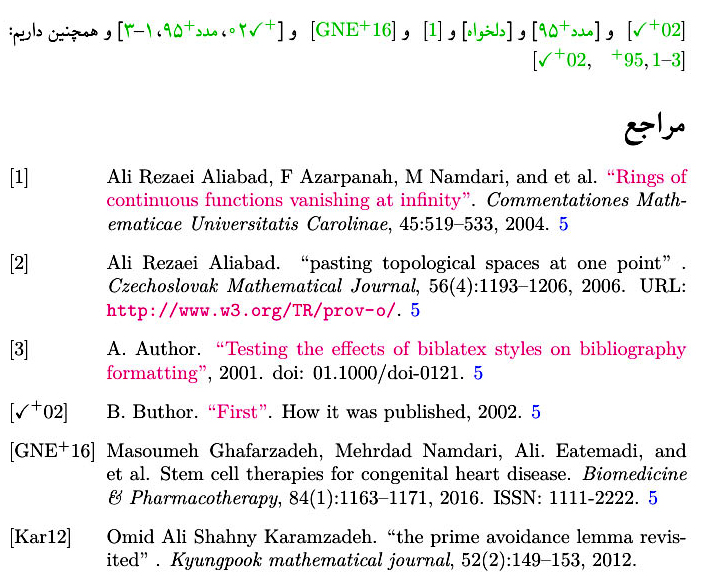
\includegraphics[width=\textwidth,height=9cm]{image/sh9}
\end{figure}
\begin{latin}
{\tt {\color{red}$\hookrightarrow$ you can sort  persian references together and also 
english \linebreak references together and  you can sort  both of them together (mixed)\linebreak too with the help of 
\verb|\noopsort| command.}}\\
{\tt\color{blue} Sample:}\\
{\color{blue}$\hookrightarrow$ Compile: XeLaTex-BibTeX-XeLaTex-XeLaTex}
\end{latin}
\begin{Verbatim}[numbers=left,fontsize=\bf,commandchars=\&\#\*,baselinestretch=1,firstnumber=1,formatcom=\color{green!50!black}]
@misc{whatever,
AUTHOR="{\noopsort{2}}{Madadpour},Ahmad ",
quotation={1},
year={2001},
chapter={5},
title={Testing the effects of bibtex styles on bibliography formatting},
murl={http://www.w3.org/TR/prov-o/},
doi={01.1000/doi-0121},
madadurltest={1},
key={665},
}
@misc{B02f,
howpublished={How it was published},
AUTHOR="{\noopsort{4}}{Madadpour},Shapour  ",
year={2002},
quotation={1},
title={First},
pages={13&raisebox#.5mm--* &!&!&!17},
madadurltest={1},
mlabel={$\checkmark^+$},
murl={http://www.w3.org/TR/prov-o/},
chapter={5},
}
@article{aliabad2004rings,
title={reference test-Rings of continuous functions vanishing at infinity},
AUTHOR= "{\noopsort{6}}{Madadpour},Alireza ",
journal={Commentationes Mathematicae Universitatis Carolinae},
volume={45},
pages={519&raisebox#.5mm--* &!&!&!533},
quotation={1},
year={2004},
murl={http://www.w3.org/TR/prov-o/},
madadurltest={1},
publisher={Charles University in Prague, Faculty of Mathematics and Physics},
}
@article{ali,
title={reference test-Pasting topological spaces at one point},
AUTHOR= "{\noopsort{8}}{Madadpour},Mahmood ",
journal={Czechoslovak Mathematical Journal},
volume={56},
number={4},
pages={1193&raisebox#.5mm--* &!&!&!1206},
quotation={1},
year={2006},
publisher={Springer},
url={http://www.w3.org/TR/prov-o/},
}
@article{Amintoosi87afzayesh,
TITLE={&prl#افزایش وضوح ناحیه‌ای*},
BOOKTITLE={&prl#چهاردهمین کنفرانس ملی سالانه انجمن کامپیوتر ایران*},
author={{\noopsort{1}}{&prl#امین‌طوسی*}&prl#محمود, * and &prl# مزینی ,ناصر*and &prl#سایرین*},
YEAR ={1387},
ORGANIZATION={&prl#دانشگاه امیرکبیر*},
ADDRESS={&prl#تهران، ایران*},
journal={&prl#نام مجله‌ی چاپ‌کننده*},
month={&prl#اسفند*},
doi={01.1000/doi-0121},
edition={&prl#ششم*},
volume={45},
number={3},
pages={101&raisebox#.5mm--* &!&!&!108},
issn={1111&raisebox#.5mm-* &!&!&!2222},
madadurltest={1},
chapter={5},
quotation={1},
LANGUAGE={Persian},
mlabel={ا.م$^+$},
slabel={$\heartsuit$},
murl={http://www.w3.org/TR/prov-o/},
}
@inbook{d,
AUTHOR={{\noopsort{1}}{&prl#مددپور*}&prl#شاپور, * and &prl# مددپور ,محمدحسین*and &prl#سایرین*},
mlabel={&prl#مدد$^+$*},
TITLE={&prl#همریختی و بروریختی در حلقه‌ها*},
JOURNAL={&prl#مجله‌ی گراف فارس*},
VOLUME={1},
YEAR={1395},
MONTH={&prl#بهار*},
PAGES={39&raisebox#.5mm--* &!&!&!43},
quotation={1},
LANGUAGE={Persian},
doi={&prl#01.1000/doi*&raisebox#.5mm-* &!&!&!0121},
isbn={123456789000},
edition={&prl#دوم*},
series={&prl#سری دوم*},
number={10},
chapter={5},
madadurltest={1},
murl={http://www.w3.org/TR/prov-o/},
publisher={&prl#انتشارات دل آهنگ*},
note={&prl#یک یادداشت اختیاری در این‌جا می‌توانید وارد کنید*},
address={‌&prl#آدرس منتشر کننده*},
slabel={$\bigstar$},
}
@phdthesis{mmm,
title={&prl#فضای توپولوژی*},
author={{\noopsort{5}}{&prl#رضایی علی‌آباد*}&prl#علی,*},
journal={Kyungpook mathematical journal},
pages={1163&raisebox#.5mm--* &!&!&!1171},
LANGUAGE ={Persian},
mlabel={&prl#ا.م.ف*},
madadurltest={1},
quotation={1},
murl={http://www.w3.org/TR/prov-o/},
series={second series},
year={2002},
url={http://www.w3.org/TR/prov-o/},
chapter={5},
school={&prl#دانشگاه چمران اهواز*},
}
@inbook{yu,
author={{\noopsort{1}}{&prl#نامداری*}&prl#مهرداد, * and &prl# کوچک‌پور ,عبدعلی*},
mlabel ={&prl#ن.ا.م$^+$*},
TITLE ={&prl#مقدمه‌ای بر نظریه‌ی  اصولی مجموعه‌ها*},
VOLUME={1},
YEAR={1394},
MONTH={&prl#بهار*},
PAGES={39&raisebox#.5mm--* &!&!&!43},
quotation={1},
LANGUAGE={Persian},
doi={322/511},
isbn={978&raisebox#.5mm-* &!&!&!600&raisebox#.5mm-* &!&!&!141&raisebox#.5mm-* &!&!&!173&raisebox#.5mm-* &!&!&!1},
edition={&prl#دوم*},
series={&prl#سری دوم*},
number={100},
chapter={5},
madadurltest={1},
murl={http://www.w3.org/TR/prov-o/},
publisher={&prl#انتشارات دانشگاه چمران*},
note={&prl#یک یادداشت اختیاری در این‌جا می‌توانید وارد کنید*},
address={&prl#آدرس منتشر کننده*},
slabel={4},
}
\end{Verbatim}
\begin{latin}
{\color{blue}$\hookrightarrow$ Compile: XeLaTex-BibTeX-XeLaTex-XeLaTex}
\end{latin}
\begin{figure}[H]
\centering
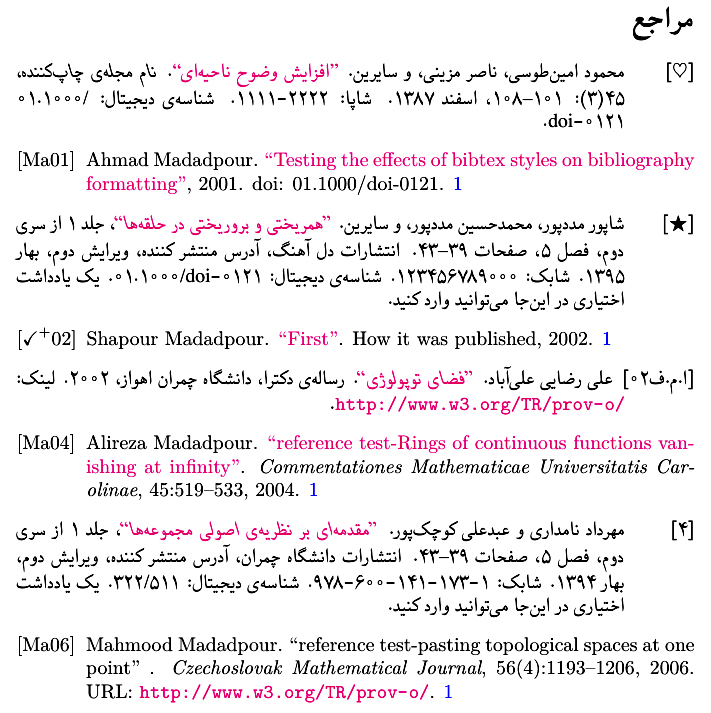
\includegraphics[width=\textwidth,height=11.5cm]{image/sh12}
\end{figure}





\noindent
\begin{latin}
{\tt{\color{blue} General example with xelatex compiler:}}\\
{\color{blue}$\hookrightarrow$ Compile: XeLaTex-BibTeX-XeLaTex-XeLaTex}
\end{latin}
\lr{\cite{B02f}}
 و
\cite{d}
و
\cite{Amintoosi87afzayesh}
و
\lr{\cite{aliabad2004rings}}
و
\lr{\cite{ghafarzadeh2016stem}}
و
\cite{aliabad2004rings,ali,whatever,B02f,d}
و همچنین داریم:
\lr{\cite{aliabad2004rings,ali,whatever,B02f,d}}

\nocite{*}                  
\bibliographystyle{alpha-persian}
%\bibliography{sample1}
%\bibliography{sample2}
%\bibliography{sample3}
%\bibliography{sample4}
%\bibliography{sample5}
%\bibliography{sample6}
%\bibliography{sample7}
\bibliography{sample8}
\newpage
\begin{latin}
\section{\lr{alpha-persian.bst with \protect \pdflatex}}
In addition to xelatex compile,
You can also use from alpha-persian.bst with pdflatex compile (without xepersian package).
To do this, just put the following codes before the  \verb|\begin{document}|.
\begin{verbatim}
\let\lr\relax
\let\setlatin\relax
\let\resetlatinfont\relax
\newenvironment{LTRbibitems}{}{}
\end{verbatim}
{\tt\color{blue} Sample:}\\
{\color{blue}$\hookrightarrow$ Compile: pdfLaTeX-BibTeX-pdfLaTeX-pdfLaTeX}
\begin{Verbatim}[numbers=left,fontsize=\bf,commandchars=\&\#\*,baselinestretch=1,firstnumber=1,formatcom=\color{green!50!black}]
@misc{whatever,
AUTHOR= "{\noopsort{1}}{Madadpour},Ahmad ",
quotation={1},
year={2001},
chapter={5},
title={Testing the effects of bibtex styles on
bibliography formatting},
murl={http://www.w3.org/TR/prov-o/},
doi={01.1000/doi-0121},
madadurltest={1},
key={665},
}
@misc{B02f,
howpublished = {How it was published},
AUTHOR= "{\noopsort{2}}{Madadpour},Shapour and
Madadpour , Mohamadhosain and Madadpour , Mitra  ",
year={2002},
quotation={1},
title={First},
pages={13--17},
madadurltest={1},
mlabel={&prl#$\checkmark^+$*},
murl={http://www.w3.org/TR/prov-o/},
chapter={5},
}
@article{aliabad2004rings,
title={reference test-Rings of continuous functions
vanishing at infinity},
AUTHOR= "{\noopsort{3}}{Madadpour},Alireza ",
journal={Commentationes Mathematicae Universitatis Carolinae},
volume={45},
pages={519--533},
quotation={1},
year={2004},
murl={http://www.w3.org/TR/prov-o/},
madadurltest={1},
publisher={Charles University in Prague, Faculty of
Mathematics and Physics},
}
@article{ali,
title={reference test-Pasting topological spaces at one point},
AUTHOR = "{\noopsort{4}}{Madadpour},Mahmood ",
journal={Czechoslovak Mathematical Journal},
volume={56},
number={4},
pages={1193--1206},
quotation={1},
year={2006},
publisher={Springer},
url={http://www.w3.org/TR/prov-o/},
}
@book{kuznetsov1998elements,
title={reference test-Elements of
applied bifurcation theory},
volume={112},
madadurltest={1},
year={1998},
edition={third},
publisher={Springer Verlag},
murl={http://www.w3.org/TR/prov-o/},
isbn={123456789000},
number={10},
pages={10--19},
series={second series},
chapter={5},
AUTHOR= "{\noopsort{5}}{Madadpour},Behrooz ",
address={The address of the publisher},
}
\end{Verbatim}
\begin{latin}
{\color{blue}$\hookrightarrow$ Compile: pdfLaTeX-BibTeX-pdfLaTeX-pdfLaTeX}
\end{latin}
\begin{figure}[H]
\centering
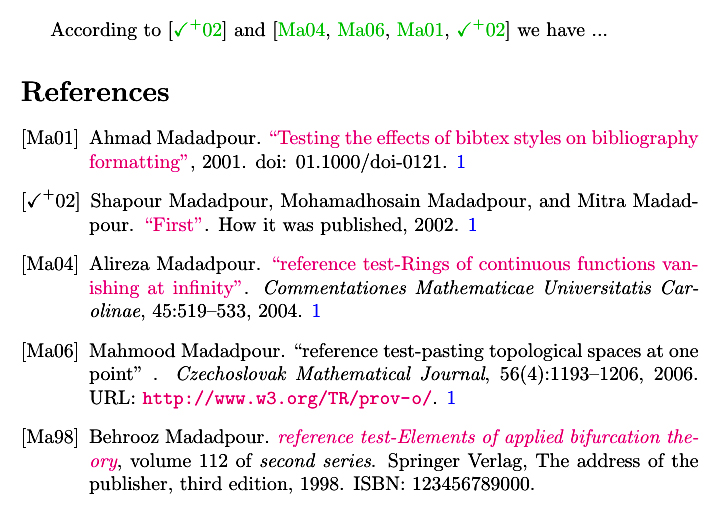
\includegraphics[width=\textwidth,height=8cm]{image/sh13}
\end{figure}
\section*{Notice}
With pdflatex compiler, we have all the properties in section \ref{12}; so enjoy it.
\end{latin}





\end{document}
In addition to latex compile,
You can also use from alpha-persian.bst with pdflatex compile(without xepersian package).
To do this, just put the following codes before the  \begin{document}.
\let\lr\relax
\let\resetlatinfont\relax
\newenvironment{LTRbibitems}{}{}


\newcommand{\pdflatex}{\LR {\leavevmode $\smash {\hbox {P\lower .6ex \hbox
				{\kern -.225em\bidi@reflect@box {D}}\hbox{\bidi@reflect@box{F}} \kern -.4em \LaTeX }}$}}
